\documentclass[../../../main.tex]{subfiles}

\begin{document}
\label{sec:methods}

In Sec. \ref{sec:teaching_philosophy}, I discussed \textit{order} and \textit{shared meaning}.  Students require PER to master the \textit{order} of physics.  Within order, there is problem-solving, analytical thinking, experimentation, and data analysis.  The students use laboratory activities to confirm concepts, and to practice analyzing graphical and numerical data.  To apply physics concepts to other disciplines (\textit{shared meaning}), students need a variety of modules and examples to form connections.  I review each type of module below in Secs. \ref{sec:per} - \ref{sec:la}.

\section{Instruction of Students in Introductory Courses}

Students are categorized as \textit{non-majors} or \textit{physics majors}.  Non-majors encounter classical physics for two semesters.  Introductory classical physics is built upon single-variable calculus, with some vector calculus introduced later.  Students not taking calculus still learn using tools from algebra and trigonometry.  \textit{Non-major} students therefore take PHYS135A/B, while those majoring in physics, engineering, math, and ICS take PHYS150/180.
\\
\vspace{0.15cm}
Three focuses are relevant for teaching at the introductory level:
\begin{enumerate}
\item \textbf{Curiosity}.  Good instruction for non-majors should \textit{entice curiosity}, which begins by encountering students' initial experience with physics.  Before the pandemic, I would give colloquia and seminars at other schools, and public lectures to children and families in East Los Angeles.  Experiencing people's curiosity forms a starting point, from which we build order.  I have given lectures at Los Nietos Middle School and colloquia here at Whittier College, and invited speakers from UC Irvine to give colloquia as well.  I planned to continue this practice at a Family Science Night at Granada Middle School, but the pandemic forced us to cancel.  Within this teaching focus, I have three measurable goals:

\begin{itemize}
\item Measurably increase student interest in physics as measured by questions 15 and 18 on the evaluation forms.
\item Teach the students to satisfy curiosity through self-designed experiments and pre-designed lab activities.
\item Coach the public speaking skills of the students to empower them to present results to peers.
\end{itemize}

\item \textbf{Improvement of Analysis Skill}.  The order within physics requires analytical skill.  Physicists help the students develop their problem-solving abilities.  We apply PER modules in introductory courses to train students, and add a healthy mixture step-by-step examples.  This involves calculations as simple as converting between units (i.e. kilograms to pounds) to plotting the trajectory of a particle in a vector field.  Within this teaching focus, I have two specific goals:

\begin{itemize}
\item Measurably increase the ability of the students to solve word problems (questions 12, 14, 19, and 20 on the evalutations).
\item Teach the students to measure with precision the correct result in laboratory settings.
\end{itemize}

\item \textbf{Applications to Society}. Our students succeed in their technical careers if they can qualitatively explain phenomenon via the shared meaning of physics.  In recent years, our OER \cite{openstax1} \cite{openstax2} have included medical and kinesiological topics.  My students engage in special units, including human muscle motion (in PHYS135A) and nerve systems (in PHYS135B and PHYS180).  The students design experiments for final projects, and sometimes these apply to their field.  One excellent example is shown in Fig. \ref{fig:taylor_1}, and several examples are included in the supporting material. Another tool is the inclusion of student-led summaries of scientific articles, which encourage class discussions about the broader implications for society.  Within this teaching focus, I have two measurable goals:

\begin{itemize}
\item Empower the students to present and discuss articles they find relevant or interesting (see Supplemental Material)
\item Manage and aid in student-designed experiments that are presented to the class (see Supplemental Material)
\end{itemize}

\end{enumerate}

\begin{figure}
\centering

\includegraphics[width=0.4\textwidth]{figures/taylor1.png}
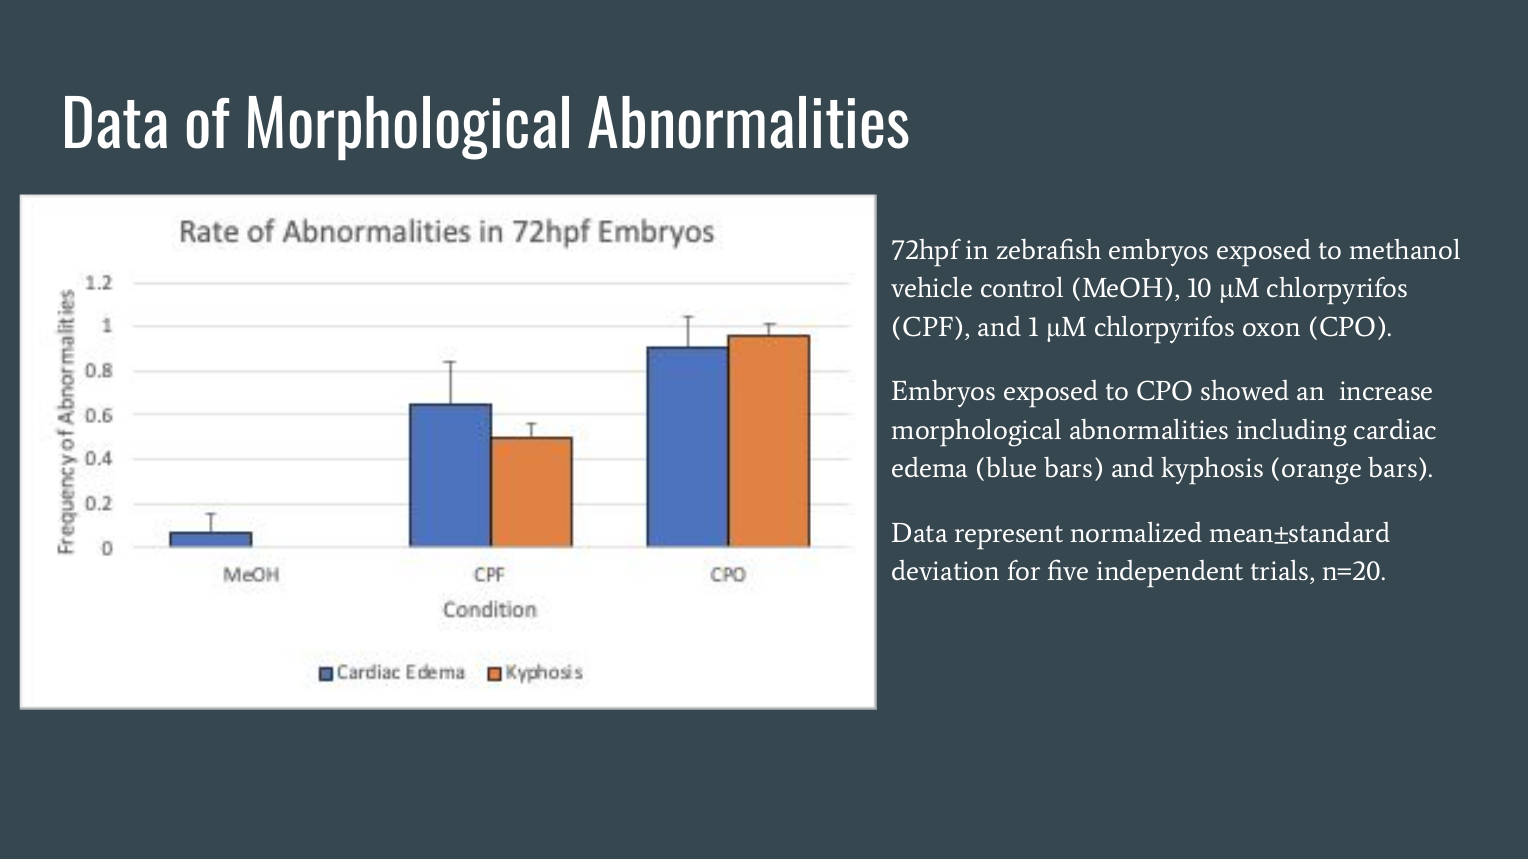
\includegraphics[width=0.4\textwidth]{figures/taylor2.png}
\caption{\label{fig:taylor_1} The title slide and key results of the final presentation of one of my students, Taylor Watanabe.  I taught this student physics for a year, followed by statistics in summer session.}
\end{figure}

\section{Instruction of Students in Advanced Courses}

\textit{Physics, ICS, and 3-2 program majors} are all students served by my department.  I have created two upper-division computer science courses that are part of the curriculum in schools similar to Whittier College, but were missing before I joined the faculty.  The first is Computer Logic and Digital Circuit Design (COSC330/PHYS306), and the second is Digital Signal Processing (DSP, COSC360) (see \cite{hmc} for an example of computer logic and \cite{rio_hondo} for an example of DSP).
\\
\vspace{0.15cm}
Three focuses are relevant for teaching physics, mathematics, and computer science majors at the advanced level:
\begin{enumerate}
\item \textbf{Mental Discipline}.  These courses require mental discipline.  The professor must foster this value in the students in two ways.  First, the students need a professional curriculum requiring \textit{analytical} and \textit{creative} thinking.  Second, the professor should demonstrate \textit{expertise} and lead the students by example.  For example, in DSP, I write computer code to illustrate graphical and computational concepts, and the students modify it for projects.  I summarize mental discipline into two goals:

\begin{itemize}
\item Challenge the students with course content that requires both analytic and creative thinking (questions 11 and 20 from the evaluation).
\item Provide the students with technical expertise and guidance (questions 12 and 19 from the evaluation).
\end{itemize}

\item \textbf{Strength in all Phases of Science}. Advanced course curriculum in physics, math, and computer science must include the following \textit{phases} of scientific activity: abstract problem solving, numerical modeling/prediction, experimental design and execution, and data analysis. I have four goals in this area, corresponding to the four phases:

\begin{itemize}
\item Measurably strengthen the abstract problem solving of the students (question 14 from evaluation).
\item Expose students to numerical modeling with computer code.
\item Assist the students with the design and execution of technical projects.
\item Strengthen the data analysis abilities of the students through technical projects.
\end{itemize}

\item \textbf{Communication}.  A critical skill in technical fields is oral and written communication.  Whittier College graduates in the fields of physics, mathematics, and computer science should be able to communicate technical ideas to their peers.  To help my advisees practice, I made the theme of my INTD100 section scientific and technical writing.  In my advanced STEM courses, the students write a longer paper and/or presentation with the goal of improvement of their technical communication.  I set two goals:

\begin{itemize}
\item Require the students to submit at least one major written or oral assignment.
\item Provide students the opportunity to refine the work in office hours before submission.
\end{itemize}
\end{enumerate}

\section{Department-Level Goals}

The Department of Physics and Astronomy has eight goals. In the coming course descriptions, these goals will be referenced.
\begin{enumerate}
\item Develop and offer a wide range of physics courses using the most effective pedagogical methods and styles.  Such courses shall include appropriate contributions to the Liberal Education Program (currently COM1 and CON2).
\item Create research experiences for physics majors that will engage and inspire them in their discovery of physics.
\item Build a departmental community that is supportive and welcoming and that encourages students in their studies of physics.
\item Keep the physics curriculum current so that students gain the skills necessary for success in today's scientific environment.
\item Teach students how to teach themselves. Give them the intellectual tools necessary for independent thinking and learning.
\item Train students to think ``scientifically'' i.e. critically, rigorously, quantitatively, and objectively, so that they can analyze problems and generate solutions.
\item Train students to effectively communicate scientific ideas to others.
\item Advise students about various career paths and help them along these paths.
\end{enumerate}

\section{Physics Education Research (PER) Modules}
\label{sec:per}

The PI and PhET modules are outlined below.
\\
\vspace{0.15cm}

\underline{PI Modules} - An active learning strategy involving group problem solving and discussion \cite{mazur2013peer} \cite{AAPTPI} \cite{PhysPort}.  Figure \ref{fig:exampleData} contains data relevant to the following example.
\begin{itemize}
\item PI-based modules contain multiple-choice questions about a physical system.  Suppose we ask the students the following question: \\ \vspace{0.5cm} \textbf{If the slope on a graph of $x(t)$ vs. $t$ is positive before $t_0$, zero at $t_0$, and negative after $t_0$, \\ \vspace{0.5cm} A) the acceleration of the object was negative before and after $t_0$.  \\ B) the acceleration of the object was positive before $t_0$, then negative. \\ C) the acceleration of the object was positive before and after $t_0$. \\ D) the object had no acceleration.}
\item Each student responds \textit{anonymously} with a device, and their answers appear on-screen (see Fig. \ref{fig:exampleData}).
\begin{figure}
\centering
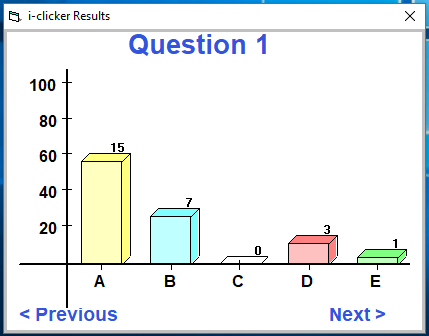
\includegraphics[width=0.45\textwidth,trim=0.15cm 1cm 0.15cm 2cm,clip=true]{figures/FirstData.PNG}
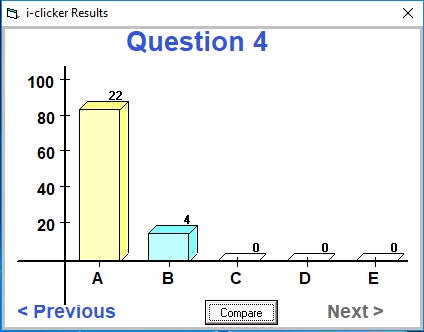
\includegraphics[width=0.45\textwidth,trim=0.15cm 1cm 0.15cm 2cm,clip=true]{figures/SecondData.PNG}
\caption{\label{fig:exampleData} (Left) An answer distribution of my 25-student PHYS135A class (A was correct).  This distribution triggered a table discussion.  One student pressed E (indicating confusion) and I took appropriate action.  (Right) After table discussions, the students responded and the fraction of correct answers was 22/25 = 0.88.}
\end{figure}
\item Students know to press E if they are confused.
\item One of two actions is taken next:
\begin{enumerate}
\item If the fraction of correct answers is $>0.7$, we proceed to the next exercise or new material\footnote{The number 0.7 was the recommended fraction at the American Association of Physics Teachers (AAPT) conference I attended in 2017.}.
\item If the fraction is $<0.7$, the professor initiates \textbf{table discussion}.
\end{enumerate}
\item \textbf{Table discussions} take place between students at the same table.  During this time the professor circulates, searching for and helping the struggling students.  After 3-5 minutes, the discussion ends.
\item A second poll of the class is taken after table discussions.  The \textit{shift} in the distribution towards the correct answer indicates improved understanding.  The professor takes appropriate action if there is not a shift.  If there are E answers, the material is re-addressed.
\item The procedure is repeated for several exercises, and table discussions take place when necessary.  After several exercises, the class proceeds to new material. See Fig. \ref{fig:exampleData} for example PI data.
\end{itemize}

\underline{PhET Modules} - These are interactive simulation tools published by The University of Colorado, Boulder \cite{phet}.  They are based on proven PER and written such that any student can operate them.
\begin{itemize}
\item The OpenStax textbooks for our courses have built-in links to PhET tools, allowing students to illustrate course concepts by visualizing and manipulating them.
\item Several HTML5-based examples are here:
\begin{enumerate}
\item Electric charge and electric field: \url{https://phet.colorado.edu/en/simulation/charges-and-fields}
\item DC circuits: \url{https://phet.colorado.edu/en/simulation/circuit-construction-kit-dc}
\end{enumerate}
\item PhET simulations are incorporated into active learning in the classroom in four situations:
\begin{enumerate}
\item When a PhET tool re-creates a laboratory measurement, it is useful and informative to first simulate the expected results and then compare to the real ones.
\item PhET tools are used when an experiment cannot be constructed in the lab, such as altering gravity or changing the friction between surfaces.  Students benefit by being able to fine-tune a system in order to understand it.
\item PhET tools are used to \textit{visualize} systems which are invisible.  Examples are magnetic, electric, and gravitational fields, which are real but not always visible.
\item In special units, such as studying the behavior of electrical signals in the human body, there are useful PhET tools from biology, chemistry, medicine, and earth science that help me engage the curiosity of students.
\end{enumerate}
\end{itemize}

\begin{figure}
\centering
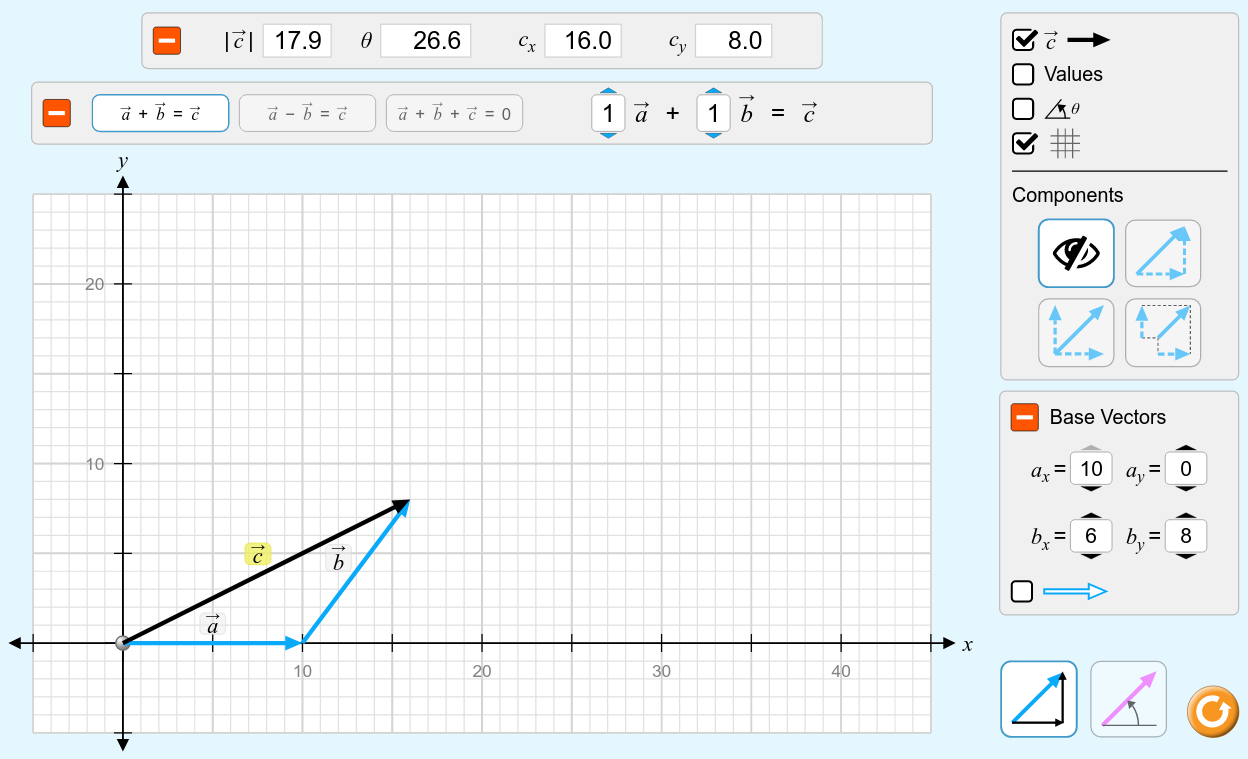
\includegraphics[width=0.4\textwidth]{figures/phet1.png}
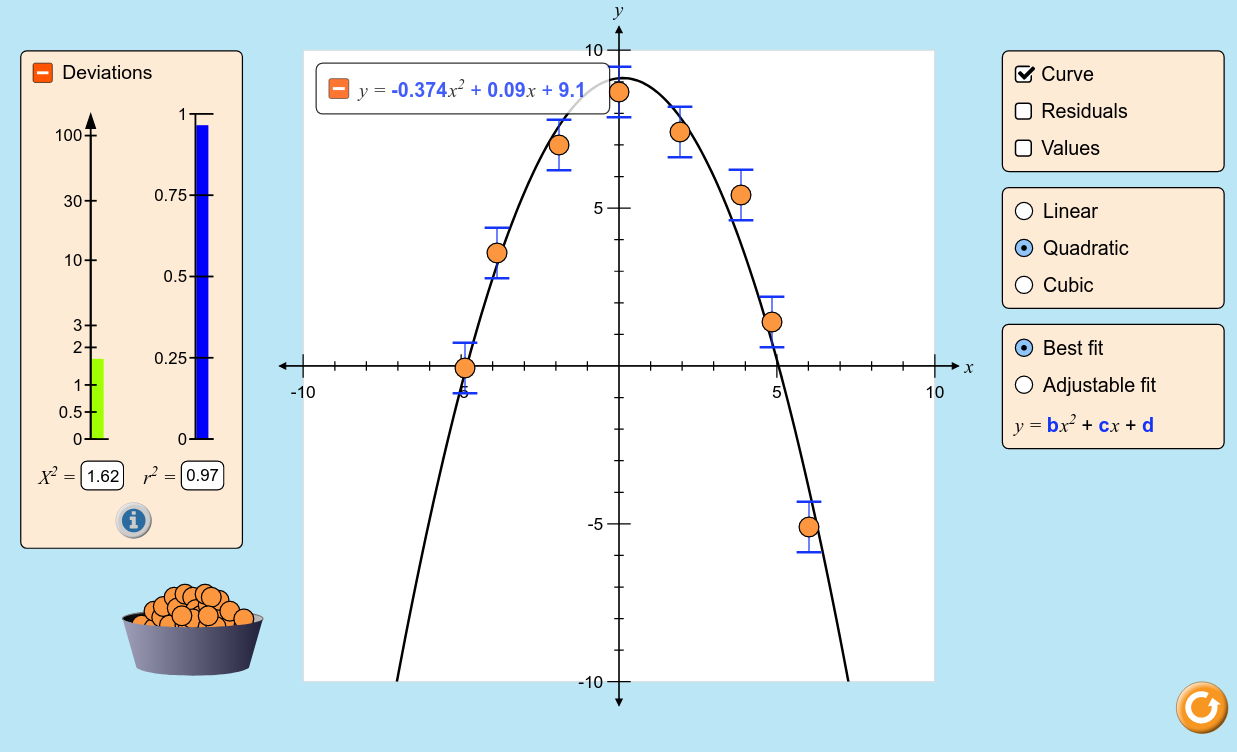
\includegraphics[width=0.4\textwidth]{figures/phet2.png}
\caption{\label{fig:phet} Two examples of PhET simulations used by my physics students in the lecture/laboratory formatted courses.  (Left) Vector addition. (Right) Curve-fitting to data.}
\end{figure}

\section{Traditional Teaching Modules}
\label{sec:tt}

Traditional teaching modules begin a warm-up exercise.  These involve topics from reading done 1-2 days before class.  An example is shown in Fig. \ref{fig:read}.  Next, we review the agenda, homework, reading schedule, and the memory bank.  The memory bank is a list of equations the students master through repeated application.  We proceed with the solution to the warm-up, and then expand to other examples.  From there, the TT ends and we proceed with a PI module, followed by either a PhET or laboratory module.  I recall the suggestion by FPC that the modules and timing should be varied.  I now include a break between the TT module and PI module, and I do vary the usage of PI, PHeT and lab activities.  During remote instruction, I created video recordings of TT modules for the students that could be downloaded via Moodle and YouTube.  The students preferred to use these for asynchronous learning and studying.

\begin{figure}
\centering
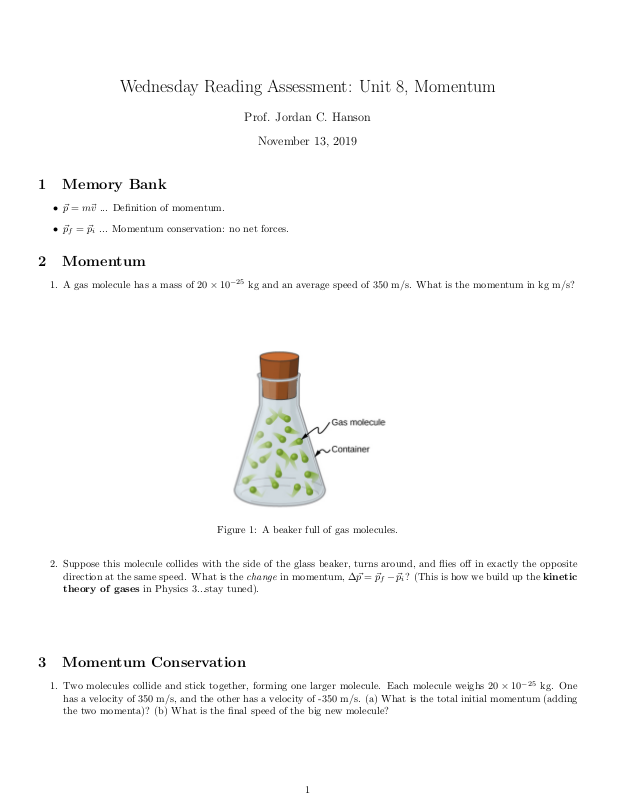
\includegraphics[width=0.45\textwidth]{figures/readingassessment.png}
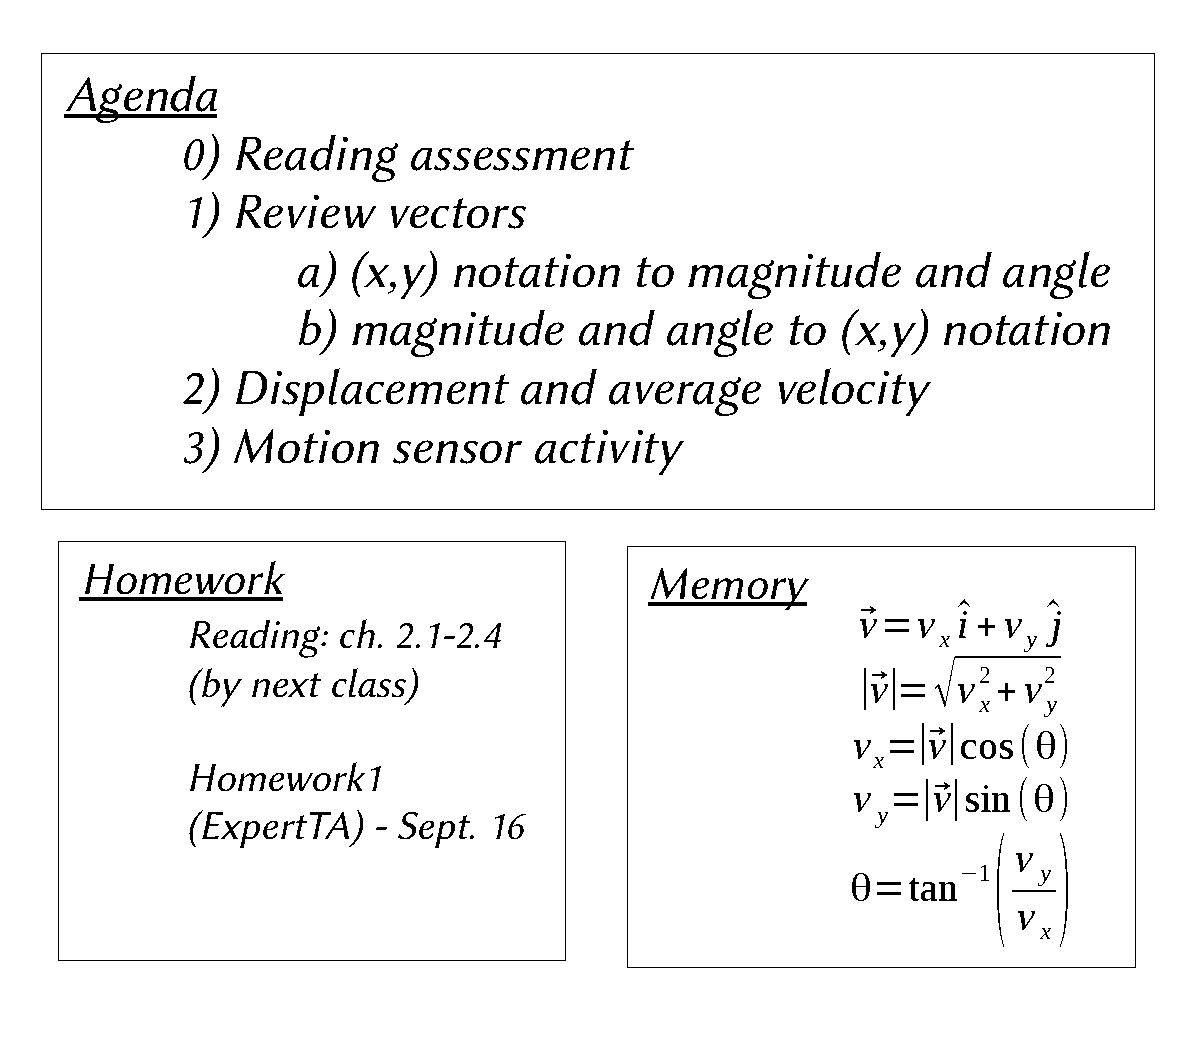
\includegraphics[width=0.45\textwidth]{ExampleTT.pdf}
\caption{\label{fig:read} (Left) An example figure from the text, integrated into my reading assessment.  (Right) The class agenda, memory bank, and homework/reading assignments are presented on the white board clearly and concisely at the beginning of class.  The reading is broken into small sections, a practice following the suggestion of a student from 2018 section.}
\end{figure}

\section{Laboratory Modules}
\label{sec:la}

Laboratory activity (LA) modules usually follow the TT and PI modules.  The students prefer to have tangible worksheets\footnote{Example included in the supporting material.}.  Philosophically, the purpose of the laboratory activities is to establish the \textit{order} through tangible experimentation.  The LA modules are done in groups.  When students are running low on energy, working together allows them learn from each other, which refreshes them and requires less energy.  During remote instruction, my department decided we valued LA modules enough to subscribe to \url{https://www.pivotinteractives.com}.  The students collect data in the same way, but they control the experiment by playing a video of an assistant operating the apparatus.  An example is shown in Fig. \ref{fig:pivot}.  Intriguingly, the students scored as well or better using online LA than in-person labs.  This is most likely due to the ``scaffolding'' of the Pivot Interactive procedures.  I continue to use LA modules with scaffolding this semester.

\begin{figure}
\centering
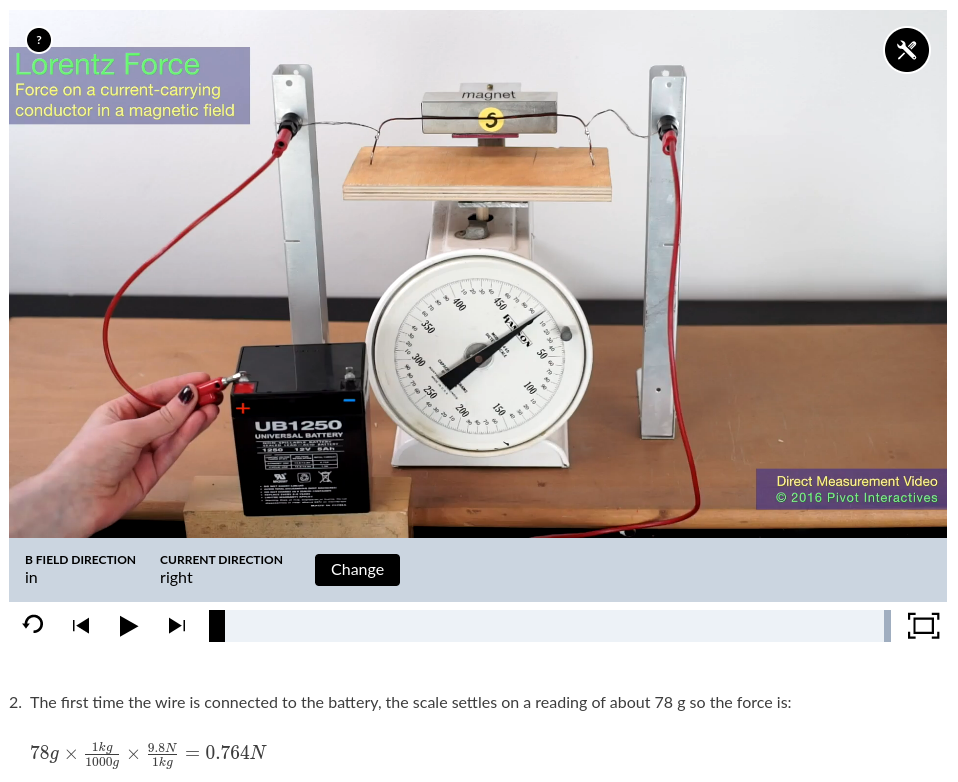
\includegraphics[width=0.5\textwidth]{figures/pivot.png}
\caption{\label{fig:pivot}  Laboratory modules are now done both in-person and through a service called Pivot Interactives.}
\end{figure}

\end{document}
